\ifx\wholebook\relax \else
% ------------------------

\documentclass[b5paper]{ctexart}
\usepackage[nomarginpar
  %, margin=.5in
]{geometry}

\addtolength{\oddsidemargin}{-0.05in}
\addtolength{\evensidemargin}{-0.05in}
\addtolength{\textwidth}{0.1in}

\usepackage[cn]{../../../prelude}

\setcounter{page}{1}

\begin{document}

\title{红黑树}

\author{刘新宇
\thanks{{\bfseries 刘新宇} \newline
  Email: liuxinyu95@gmail.com \newline}
  }

\maketitle
\fi

\markboth{红黑树}{基本算法}

\ifx\wholebook\relax
\chapter{红黑树}
\numberwithin{Exercise}{chapter}
\fi

第二章的例子使用二叉搜索树来统计文章中单词的频次。能否用它来处理通讯录、查询联系人呢?如下面的例子所示:

\lstset{frame = single}
\begin{lstlisting}[language=Bourbaki]
void addrBook(Input in) {
    Map<String, String> dict
    while (String name, String addr) = read(in) {
        dict[name] = addr
    }
    loop {
        string name = read(Console)
        var addr = dict[name]
        if (addr == null) {
            print("not found")
        } else {
            print("address: ", addr)
        }
    }
}
\end{lstlisting}

但这个方法性能不佳,尤其是搜索Zara、Zed、Zulu等姓名时更加明显。通讯录是按照字典顺序排列的。如果依次把1, 2, 3, ..., $n$插入二叉搜索树,就会得到\cref{fig:unbalanced-tree}中的结果。对于高为$h$的二叉搜索树,查找的复杂度为$O(h)$。如果树比较平衡,我们就能够达到$O(\lg n)$的性能。但在这一极端情况下,查找的性能退化为$O(n)$。等同于列表扫描。

\begin{figure}[htbp]
  \centering
  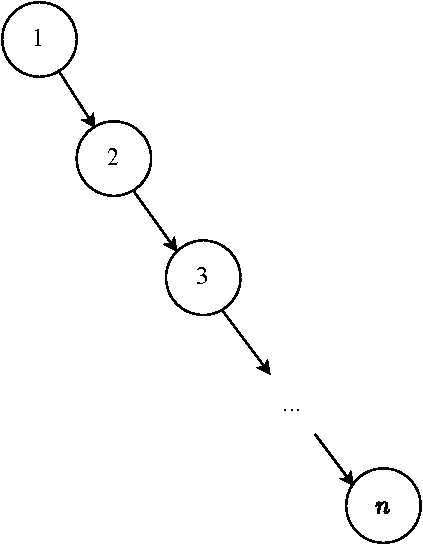
\includegraphics[scale=0.5]{img/unbalanced}
  \caption{不平衡的树} \label{fig:unbalanced-tree}
\end{figure}

\begin{Exercise}\label{ex:rbt-unbalance}
\Question{对于较大的通讯录,为了加快构建速度,可以使用两个并发的任务:一个从头部向后,另外一个从后向前读取。当两个任务相遇时结束。这样构建出的二叉搜索树是什么样子的?如果把通讯录分成更多片断,使用多任务会得到什么结果?参考\cref{fig:unbalanced-trees},找出更多的不平衡情况。}
\end{Exercise}

\begin{Answer}[ref = {ex:rbt-unbalance}]
\Question{对于较大的通讯录,为了加快构建速度,可以使用两个并发的任务:一个从头部向后,另外一个从后向前读取。当两个任务相遇时结束。这样构建出的二叉搜索树是什么样子的?如果把通讯录分成更多片断,使用多任务会得到什么结果?参考\cref{fig:unbalanced-trees},找出更多的不平衡情况。

\vspace{3mm}
由于通讯录按照字典顺序排列,头尾两个任务分别产生两棵不平衡树。头:$T_h = ((...(\nil, k_1, \nil), ...), k_m, \nil)$, 尾:$T_t = (\nil, k_{m+1}, (\nil, k_{m+2}, ... (\nil, k_n, \nil))...)$。形如\cref{fig:unbalanced-trees}(c)。如果分成多个片段,每个任务产生一个如$T_h$形状的子树。这些子树组合在一起成为一棵非平衡树。\cref{fig:unbalanced-trees}(b)在构建时,元素大小交错,每个节点都有一个空分枝。}
\end{Answer}

\begin{figure}[htbp]
  \centering
  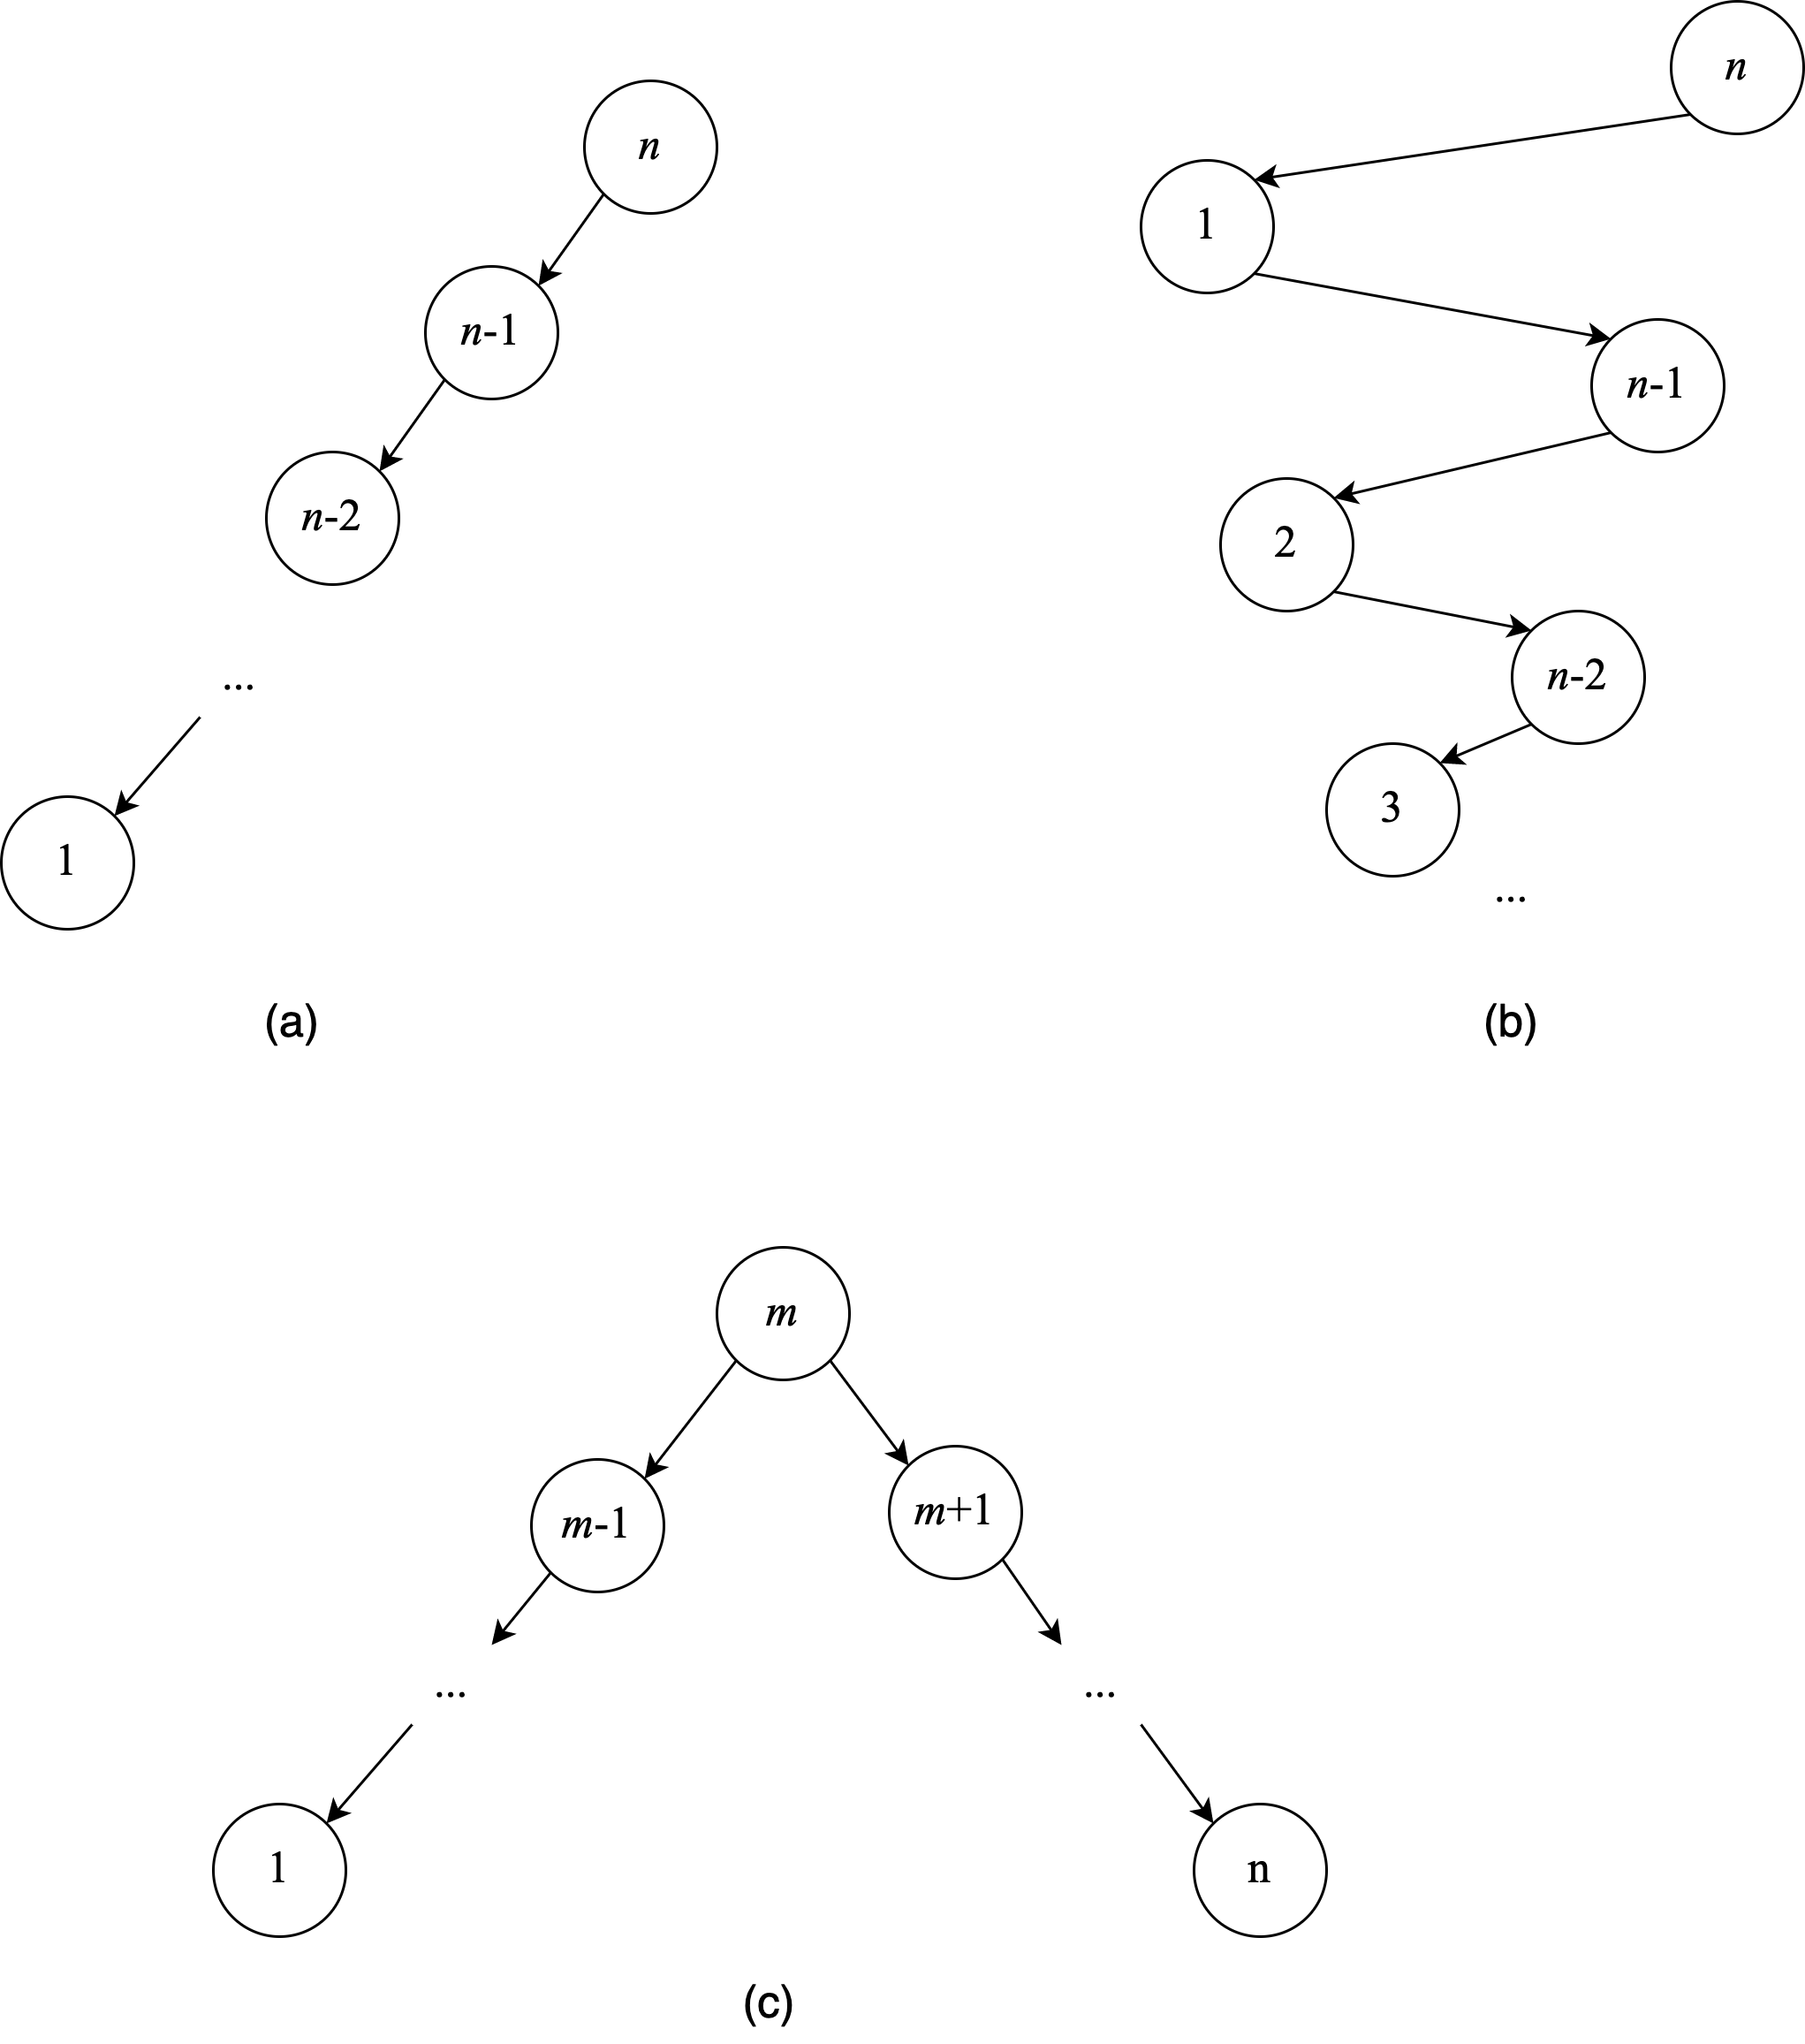
\includegraphics[scale=0.5]{img/unbalanced-trees}
  \caption{一些不平衡的二叉树}
  \label{fig:unbalanced-trees}
\end{figure}

\section{平衡}

\index{树旋转}
为避免极不平衡的情况,可将输入序列打乱(\cref{sec:bst-random-build})。但这种方法有局限性,无法处理交互输入的序列。人们找到了一些解决平衡性的方法,它们大多依赖二叉树的旋转操作。旋转操作可以在改变树结构的同时保持元素有序。本章介绍红黑树,一种常见的自平衡二叉搜索树。下一章介绍另一种自平衡树——AVL树。第8章还会介绍伸展树,它能够随着操作,逐步恢复平衡。存在不同的二叉树产生相同的的中序遍历结果。树旋转保持中序遍历结果不变,如\cref{fig:tree-rotation}所示。旋转操作可以通过模式匹配来定义:

\begin{figure}[htbp]
  \centering
  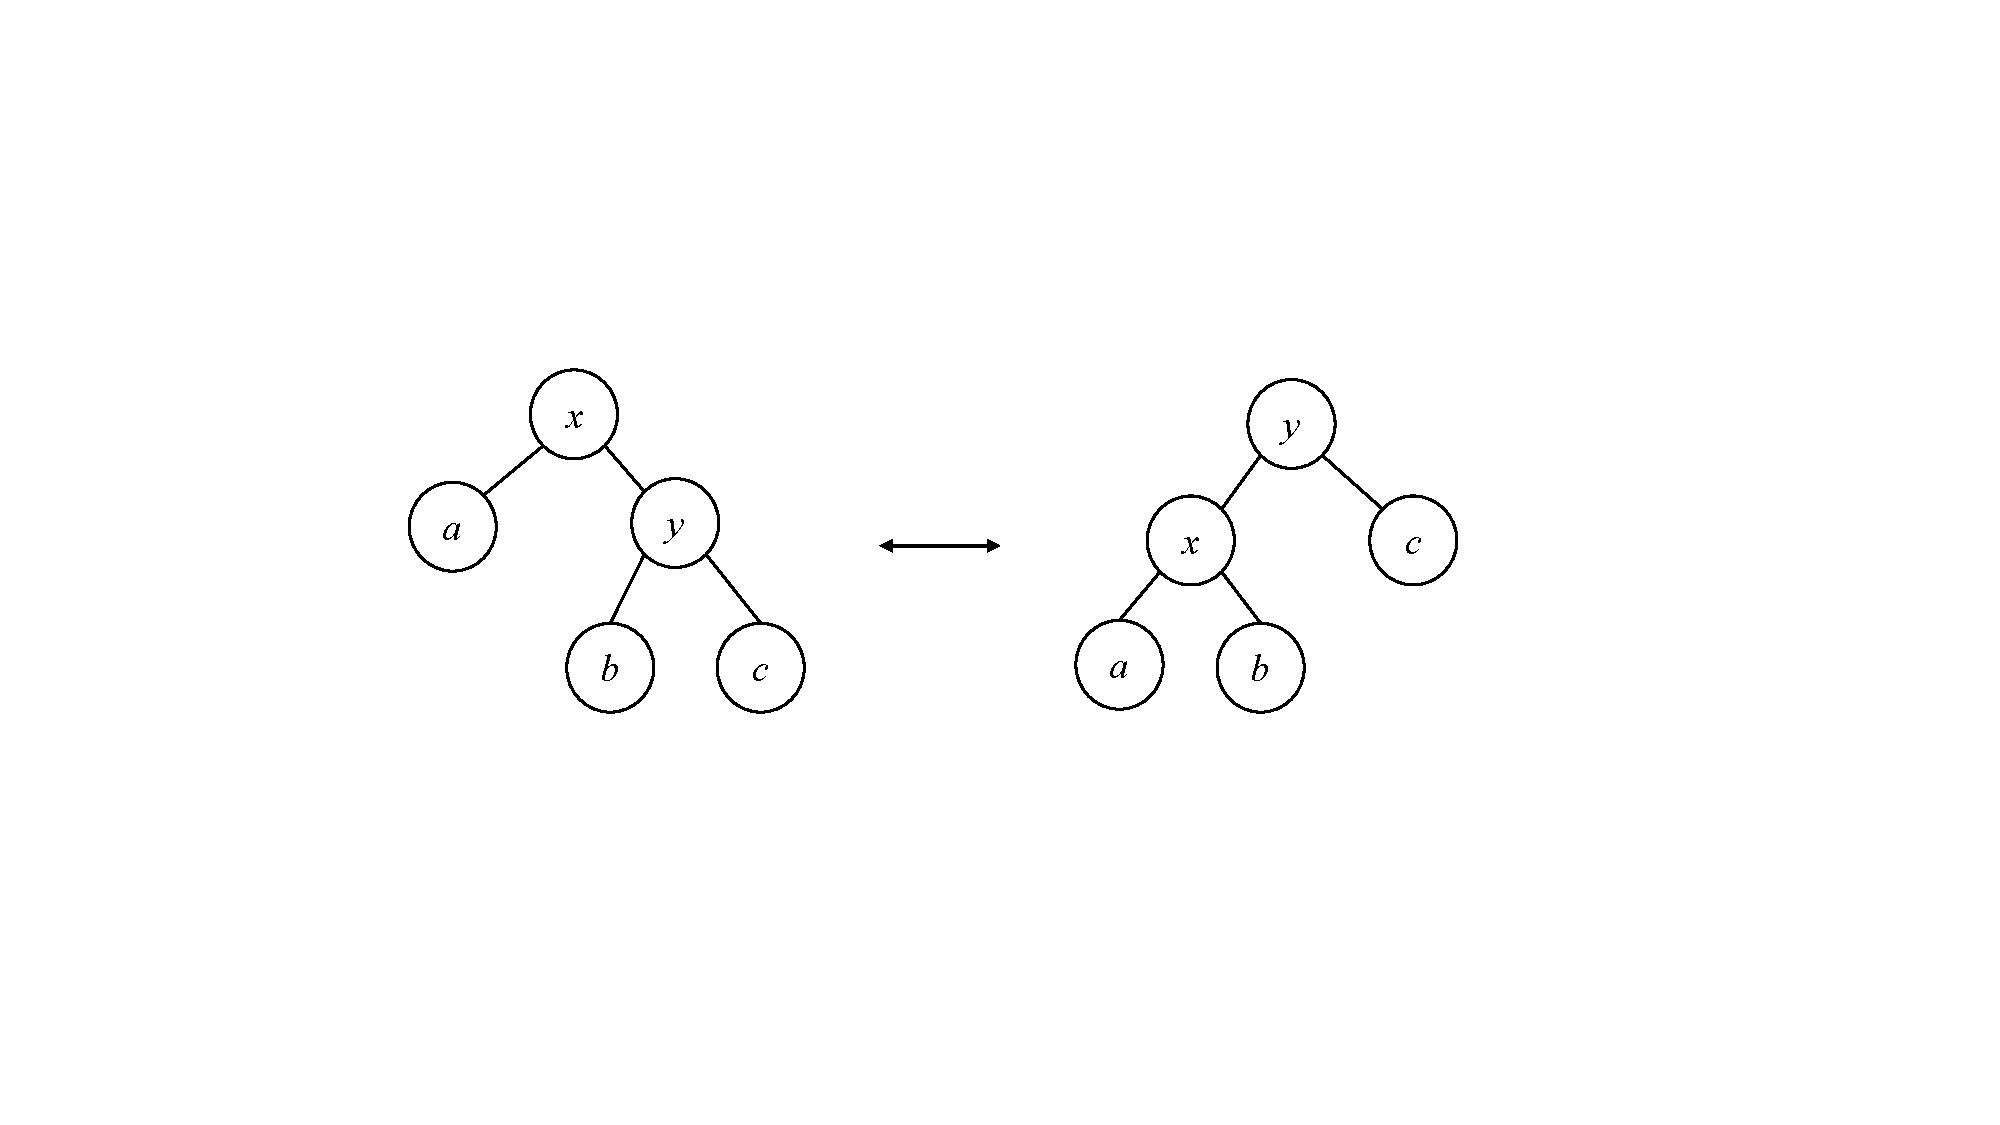
\includegraphics[scale=0.4, page=1]{img/rbtree}
  \caption{树的左右旋转}
  \label{fig:tree-rotation}
\end{figure}

\be
\begin{array}{rcl}
rotate_l\ (a, x, (b, y, c)) & = & ((a, x, b), y, c)) \\
rotate_l\ T & = & T \\
\end{array}
\ee

和

\be
\begin{array}{rcl}
rotate_r\ ((a, x, b), y, c) & = & (a, x, (b, y, c)) \\
rotate_r\ T & = & T \\
\end{array}
\ee

如果模式没有匹配(例如两棵子树都为空),每个式子的第二行保持树不变。旋转操作也可以通过一系列步骤实现。我们需要将子树和父引用设置正确。在旋转时,我们传入根节点$T$和要旋转的子树$x$:

\begin{algorithmic}[1]
\Function{Left-Rotate}{$T, x$}
  \State $p \gets$ \Call{Parent}{$x$}
  \State $y \gets$ \Call{Right}{$x$} \Comment{设$y \ne$ NIL}
  \State $a \gets$ \Call{Left}{$x$}
  \State $b \gets$ \Call{Left}{$y$}
  \State $c \gets$ \Call{Right}{$y$}
  \State \Call{Replace}{$x, y$}  \Comment{用$y$替换$x$}
  \State \Call{Set-Subtrees}{$x, a, b$} \Comment{令$a, b$为$x$的子树}
  \State \Call{Set-Subtrees}{$y, x, c$} \Comment{令$x, c$为$y$的子树}
  \If{$p = $ NIL}  \Comment{此前$x$是根节点}
    \State $T \gets y$
  \EndIf
  \State \Return $T$
\EndFunction
\end{algorithmic}

右旋\textproc{Right-Rotate}的实现是对称的,我们将其留作练习。\textproc{Replace}($x$, $y$)使用$y$替换$x$:

\begin{algorithmic}[1]
\Function{Replace}{$x, y$}
  \State $p \gets$ \Call{Parent}{$x$}
  \If{$p$ = NIL} \Comment{$x$是根节点}
    \If{$y \ne$ NIL}
           \Call{Parent}{$y$} $\gets$ NIL
    \EndIf
  \ElsIf{\Call{Left}{$p$} $= x$}
    \State \Call{Set-Left}{$p$, $y$}
  \Else
    \State \Call{Set-Right}{$p$, $y$}
  \EndIf
  \State \Call{Parent}{$x$} $\gets$ NIL
\EndFunction
\end{algorithmic}

\textproc{Set-Subtrees}($x, L, R$)将$L$设为$x$的左子树,$R$设为右子树:

\begin{algorithmic}[1]
\Function{Set-Subtrees}{$x, L, R$}
  \State \Call{Set-Left}{$x, L$}
  \State \Call{Set-Right}{$x, R$}
\EndFunction
\end{algorithmic}

它进一步调用\textproc{Set-Left}和\textproc{Set-Right}完成子树的设置:

\begin{algorithmic}[1]
\Function{Set-Left}{$x, y$}
  \State \Call{Left}{$x$} $\gets y$
  \If{$y \ne$ NIL}
    \Call{Parent}{$y$} $\gets x$
  \EndIf
  \EndFunction

\Statex

\Function{Set-Right}{$x, y$}
  \State \Call{Right}{$x$} $\gets y$
  \If{$y \ne$ NIL}
    \Call{Parent}{$y$} $\gets x$
  \EndIf
\EndFunction
\end{algorithmic}

通过对比,可以看到模式匹配如何简化树旋转的实现。从这一点出发冈崎在1995年实现了红黑树的纯函数式算法\cite{okasaki}。

\begin{Exercise}\label{ex:rbt-right-rotate}
\Question{实现右旋\textproc{Right-Rotate}操作。}
\end{Exercise}

\begin{Answer}[ref = {ex:rbt-right-rotate}]
\Question{实现右旋\textproc{Right-Rotate}操作。

\begin{algorithmic}[1]
\Function{Right-Rotate}{$T, y$}
  \State $p \gets$ \Call{Parent}{$y$}
  \State $x \gets$ \Call{Left}{$y$} \Comment{设$x \neq$ NIL}
  \State $a \gets$ \Call{Left}{$x$}
  \State $b \gets$ \Call{Right}{$x$}
  \State $c \gets$ \Call{Right}{$y$}
  \State \Call{Replace}{$y, x$}  \Comment{用$x$替换$y$}
  \State \Call{Set-Subtrees}{$y, b, c$} \Comment{令$b, c$为$y$的子树}
  \State \Call{Set-Subtrees}{$x, a, y$} \Comment{令$a, y$为$x$的子树}
  \If{$p = $ NIL}  \Comment{此前$y$是根节点}
    \State $T \gets x$
  \EndIf
  \State \Return $T$
\EndFunction
\end{algorithmic}
}
\end{Answer}

\section{定义}
\index{红黑树}

红黑树是一种自平衡二叉搜索树\cite{wiki-rbt}。它是2-3-4树的等价形式\footnote{第7章,B树。对于任一2-3-4树,都存在至少一棵红黑树,其元素顺序相同。}。通过对节点进行着色和旋转,红黑树可以高效地保持平衡。我们在二叉搜索树的定义上给节点赋予红、黑颜色。我们称一棵树为红黑树,如果它满足下面5条性质\cite{CLRS}:

\index{红黑树!红黑性质}
\begin{enumerate}
\item 节点的颜色为红色或黑色。
\item 根节点为黑色。
\item 所有NIL节点为黑色。
\item 如果一个节点为红色,则它的两个子节点都是黑色。
\item 从任一节点出发到所有叶子节点的路径上包含相同数量的黑色节点。
\end{enumerate}

为什么这5条性质能保证红黑树的平衡性呢?关键在于:从根节点出发到达叶节点的所有路径中,最长路径不会超过最短路径两倍。性质4保证了不存在两个连续的红色节点。因此,最短的路径只含有黑色的节点。任何更长的路径一定含有红色节点。根据性质5,从任何节点出发的所有的路径都含有相同数量的黑色节点,自然这条对于根节点也成立。这就最终保证了没有任何路径超过最短路径长度的两倍\cite{wiki-rbt}。\cref{fig:rbt-example-with-nil}的例子展示了一棵红黑树。

\begin{figure}[htbp]
  \centering
  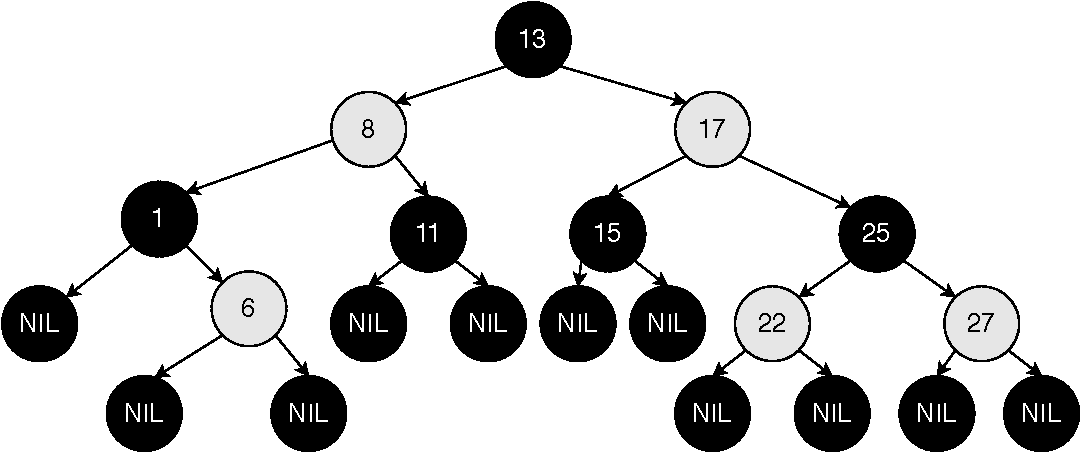
\includegraphics[scale=0.5]{img/rbt-example-with-nil}
  \caption{红黑树}
  \label{fig:rbt-example-with-nil}
\end{figure}

由于所有的NIL节点都是黑色的,我们通常将NIL节点隐藏不画出,如\cref{fig:rbt-example}所示。所有不改变树结构的操作都和二叉搜索树相同,包括查找、最大、最小值等。只有插入和删除操作是特殊的。下面的例子程序在二叉搜索树的基础上增加了颜色定义。我们记空树为$\nil$,否则记为$(c, l, k, r)$,分别表示颜色$c$(红/黑)、元素$k$,左右子树$l$、$r$。

\begin{figure}[htbp]
  \centering
  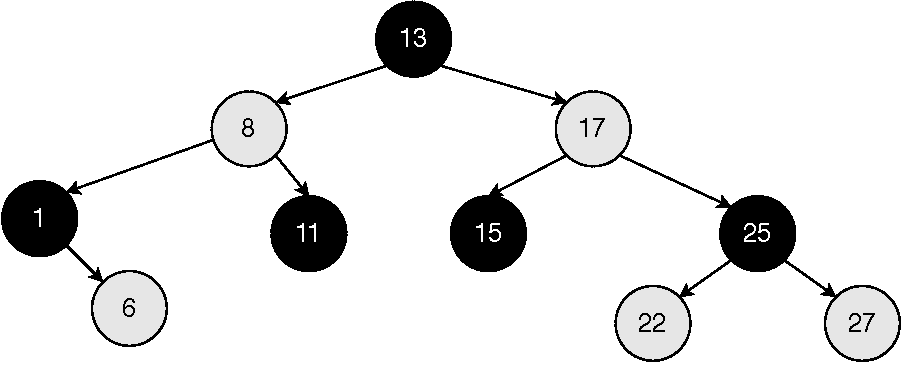
\includegraphics[scale=0.5]{img/rbt-example}
  \caption{隐藏NIL节点}
  \label{fig:rbt-example}
\end{figure}

\begin{Haskell}
data Color = R | B
data RBTree a = Empty | Node Color (RBTree a) a (RBTree a)
\end{Haskell}

\begin{Exercise}\label{ex:rbt-bounds}
\Question{证明含有$n$个节点的红黑树,其高度$h$不会超过$2 \lg (n+1)$。}
\end{Exercise}

\begin{Answer}[ref = {ex:rbt-bounds}]
\Question{证明含有$n$个节点的红黑树,其高度$h$不会超过$2 \lg (n+1)$。

我们首先引入“黑色高度”的定义。节点$x$的黑色高度$bh(x)$是从$x$(不含$x$)到某一叶子节点路径上的黑色节点数目。根据红黑树的性质5,所有路径包含相同数量的黑色节点。所以这一定义是有效的。特别地,称根结点的黑色高度为红黑树的黑色高度。

\begin{proof}
我们首先证明以任何节点$x$为根的子树至少包含$2^{bh(x)} - 1$个节点。我们对$x$的高度使用数学归纳法:若高度为0,则$x =$ NIL,子树至少含有$2^0 - 1 = 0$个节点。现在考虑分枝节点$x$,它的左右子树的黑色高度是$bh(x)$(子树的根为黑色)或$bh(x) - 1$(子树的根为红色)。由于$x$的子树高度一定小于$x$的高度,根据归纳假设,每棵子树至少含有$2^{bh(x) - 1} - 1$个节点。所以子树$x$至少含有:$2(2^{bh(x) - 1} - 1) + 1 = 2^{bh(x)} - 1$个节点。

令红黑树的高度为$h$,根据红黑树性质4,不存在连续的红色节点。所以任一路径上,黑色节点的数目超过一半。因此红黑树的黑色高度至少为$h/2$。因此:

\[
n \geq 2^{h/2} - 1 \Rightarrow 2^{h/2} \leq n + 1
\]
两边取对数得到:$h/2 \leq \lg (n + 1)$,即:$h \leq 2 \lg (n + 1)$。
\end{proof}
}
\end{Answer}

\section{插入}
\index{红黑树!插入}

插入算法包含两个步骤:第一步和二叉搜索树相同,树可能会变得不再平衡;第二步修复红黑树的颜色性质。插入时,我们令新节点为红色。只要它不是根节点,除了第四条外的所有性质都可以满足。唯一的问题是可能引入两个相邻的红色节点,共有4种情况需要修复。它们具有统一的形式\cite{okasaki},如\cref{fig:insert-fix}所示。

\begin{figure}[htbp]
  \centering
  \includegraphics[scale=0.4, page=2]{img/rbtree}
  \caption{插入后需要修复的四种情况}
  \label{fig:insert-fix}
\end{figure}

四种情况都把红色向上移动一层。如果进行自底向上的递归修复,可能会把根节点染成红色。根据性质2,最后需要把根节点变回黑色。利用模式匹配,我们定义$balance$函数修复平衡。令节点的颜色变量为$\mathcal{C}$,取值为黑色$\mathcal{B}$或红色$\mathcal{R}$。

\be
\begin{array}{rcl}
%\text{up left:} & & \\
balance\ \mathcal{B}\ (\mathcal{R}, (\mathcal{R}, a, x, b), y, c)\ z\ d & = & (\mathcal{R}, (\mathcal{B}, a, x, b), y, (\mathcal{B}, c, z, d)) \\
%\text{up right:} & & \\
balance\ \mathcal{B}, (\mathcal{R}, a, x, (\mathcal{R}, b, y, c))\ z\ d  & = & (\mathcal{R}, (\mathcal{B}, a, x, b), y, (\mathcal{B}, c, z, d)) \\
%\text{bottom left:} & & \\
balance\ \mathcal{B}\ a\ x\ (\mathcal{R}, b, y, (\mathcal{R}, c, z, d)) & = & (\mathcal{R}, (\mathcal{B}, a, x, b), y, (\mathcal{B}, c, z, d))  \\
%\text{bottom right:} & & \\
balance\ \mathcal{B}\ a\ x\ (\mathcal{R}, (\mathcal{R}, b, y, c), z, d) & = & (\mathcal{R}, (\mathcal{B}, a, x, b), y, (\mathcal{B}, c, z, d))  \\
%\text{otherwise:} & & \\
balance\ T & = & T \\
\end{array}
\ee

如果四种模式都不满足,最后一行保证此时不会改变树的形状。红黑树的插入算法定义为:$insert\ x\ T = makeBlack\ (ins\ x\ T)$,或写成柯里化的形式:

\be
insert x = makeBlack \circ ins\ x
\ee

其中:

\be
\begin{array}{rcl}
ins\ x\ \nil\ & = & (\mathcal{R}, \nil, x, \nil) \\
ins\ x\ (\mathcal{C}, l, k, r) & = & \begin{cases}
  x < k: & balance\ \mathcal{C}\ (ins\ x\ l)\ k\ r \\
  x > k: & balance\ \mathcal{C}\ l\ k\ (ins\ x\ r) \\
  \end{cases}
\end{array}
\ee

如果树为空,我们创建一个值为$x$的红色叶子节点;否则比较$x$和$k$的大小,递归地将$x$插入到子树中。然后用$balance$修复平衡性。最后强制把根节点染成黑色。

\be
makeBlack\ (\mathcal{C}, l, k, r) = (\mathcal{B}, l, k, r)
\ee

下面是对应的例子程序:

\begin{Haskell}
insert x = makeBlack . (ins x) where
    ins x Empty = Node R Empty x Empty
    ins x (Node color l k r)
        | x < k     = balance color (ins x l) k r
        | otherwise = balance color l k (ins x r)
    makeBlack (Node _ l k r) = Node B l k r

balance B (Node R (Node R a x b) y c) z d = Node R (Node B a x b) y (Node B c z d)
balance B (Node R a x (Node R b y c)) z d = Node R (Node B a x b) y (Node B c z d)
balance B a x (Node R b y (Node R c z d)) = Node R (Node B a x b) y (Node B c z d)
balance B a x (Node R (Node R b y c) z d) = Node R (Node B a x b) y (Node B c z d)
balance color l k r = Node color l k r
\end{Haskell}

我们略去了重复值的处理。如果要插入的值已经存在,我们可以覆盖或丢弃,还可以在节点中用一个列表存储相应的数据(\cite{CLRS},269页)。\cref{fig:insert-example}给出了两棵红黑树。它们分别由序列11, 2, 14, 1, 7, 15, 5, 8, 4和1, 2, ..., 8构建而成。第二个例子说明,即使序列已序,红黑树仍然保持平衡。

\begin{figure}[htbp]
  \centering
  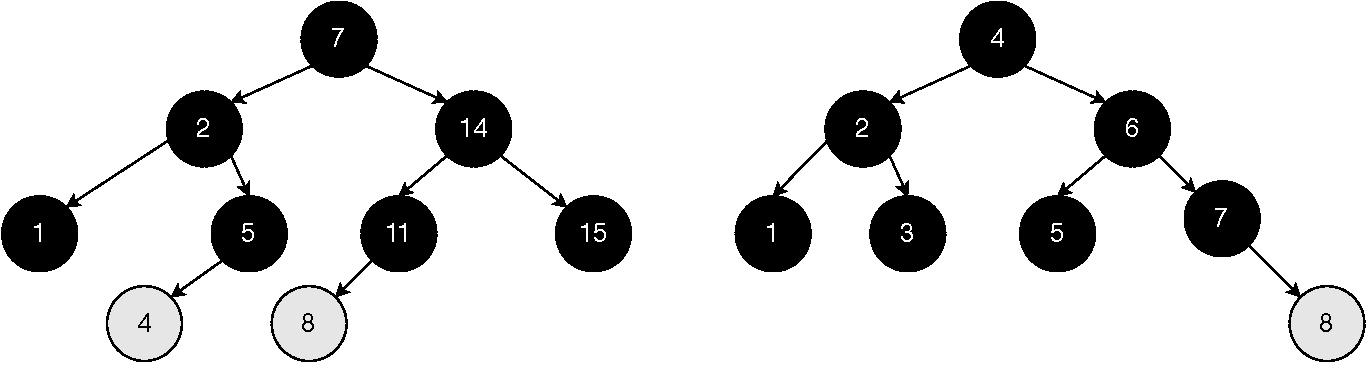
\includegraphics[scale=0.5]{img/insert-haskell}
  \caption{插入产生的红黑树}
  \label{fig:insert-example}
\end{figure}

算法自顶向下递归地进行插入和修复,对于高度为$h$的树,其复杂度为$O(h)$。由于我们始终维护红黑树的颜色性质,$h$和节点个数$n$呈对数关系。插入算法的复杂度为$O(\lg n)$。

\begin{Exercise}\label{ex:rbt-insert-wo-pm}
\Question{不使用模式匹配,分别检查四种情况实现$insert$算法。}
\end{Exercise}

\begin{Answer}[ref = {ex:rbt-insert-wo-pm}]
\Question{不使用模式匹配,分别检查四种情况实现$insert$算法。
\begin{Bourbaki}
Node<T> insert(Node<T> t, T x) = makeBlack(ins(t, x))

Node<T> makeBlack(Node<T> t) {
    t.color = Color.BLACK
    return t
}

Node<T> ins(Node<T> t, T x) {
    if t == null then return Node(null, x, null, Color.BLACK)
    return if x < t.key
           then balance(t.color, ins(t.left, x), t.key, t.right)
           else balance(t.color, t.left, t.key, ins(t.right, x))
}

Node<T> balance(Color c, Node<T> l, T k, Node<T> r) {
    return if c == Color.BLACK {
        if isRed(l) and isRed(l.left) {
            Node(Node(l.left.left, l.left.key, l.left.right, Color.BLACK),
                 l.key,
                 Node(l.right, k, r, Color.BLACK),
                 Color.RED)
        } else if isRed(l) and isRed(l.right) {
            Node(Node(l.left, l.key, l.right.left, Color.BLACK),
                 l.right.key,
                 Node(l.right.right, k, r, Color.BLACK),
                 Color.RED)
        } else if isRed(r) and isRed(r.right) {
            Node(Node(l, k, r.left, Color.BLACK),
                 r.key,
                 Node(r.left.right, r.right.key, r.right.right, Color.BLACK),
                 Color.RED)
        } else if isRed(r) and isRed(r.left) {
            Node(Node(l, k, r.left.left, Color.BLACK),
                 r.left.key,
                 Node(r.left.right, r.key, r.right, Color.BLACK),
                 Color.RED)
        } else {
            Node(l, k, r, c)
        }
    } else {
        Node(l, k, r, c)
    }
}

Bool isRed(Node<T> t) = (t != null and t.color == Color.RED)
\end{Bourbaki}
}
\end{Answer}

\section{删除}
\index{红黑树!删除}

红黑树的删除比插入复杂。也可以通过模式匹配和递归简化删除\footnote{实际上通过重用不变的部分重新构建了树。这一特性称作persist}的实现。我们还可以利用其它方式来达到删除的效果。例如,一次性构建一棵树,用于后继的多次查找\cite{okasaki-blog}。删除时在节点上加一个标记,当带有标记的节点超过50\%时,用未标记的节点重建一棵树。删除也会破坏红黑树的性质,需要进行修复。问题只发生在删除黑色节点时违反性质5,使得某一路径上的黑色节点数目少于其它的路径。我们引入“双重黑色”(\cite{CLRS},290页)节点来恢复第五条性质。一个这样的节点算作两个黑色节点。删除黑色节点$x$时,我们将黑色向上移动到父节点,或者向下移动到子树上。令接受黑色的节点为$y$。如果$y$原来是红色,将其变为黑色;如果$y$原来是黑色,则变为“双重黑色”,记作$\mathcal{B}^2$。下面的例子程序增加了双重黑色的定义:

\begin{Haskell}
data Color = R | B | BB
data RBTree a = Empty | BBEmpty | Node Color (RBTree a) a (RBTree a)
\end{Haskell}

由于所有的空节点(NIL)都是黑色,当将黑色移动到空节点时,其变为“双重黑色”空节点(\texttt{BBEmpty}或加粗的$\pmb{\varnothing}$)。删除时,第一步和普通二叉搜索树相同;如果被删除节点是黑色的,接下来进行修复:

\be
delete\ x = makeBlack \circ del\ x
\ee

这一定义是柯里化的。如果树中只有一个元素,删除后它变为空。为了处理这一情况,我们需要修改$makeBlack$的定义如下:

\be
\begin{array}{rcl}
makeBlack\ \nil & = & \nil \\
makeBlack\ (\mathcal{C}, l, k, r) & = & (\mathcal{B}, l, k, r) \\
\end{array}
\ee

$del$接受要删除的元素$x$和一棵树:

\be
\resizebox{\linewidth}{!}{\ensuremath{
\begin{array}{rcl}
del\ x\ \nil\ & = & \nil \\
del\ x\ (\mathcal{C}, l, k, r) & = & \begin{cases}
  x < k: & fixB^2(\mathcal{C}, (del\ x\ l), k, r) \\
  x > k: & fixB^2(\mathcal{C}, l, k, (del\ x\ r)) \\
  x = k: & \begin{cases}
    l = \nil: & \text{if}\ \mathcal{C} = \mathcal{B}\ \text{then}\ shiftB\ r\ \text{else}\ r \\
    r = \nil: & \text{if}\ \mathcal{C} = \mathcal{B}\ \text{then}\ shiftB\ l\ \text{else}\ l \\
    \text{否则}: & fixB^2(\mathcal{C}, l, m, (del\ m\ r)), \text{其中}: m = min(r) \\
  \end{cases}
\end{cases}
\end{array}
}}
\ee

如果树为空,结果为$\nil$;否则我们比较$x$和树中的$k$,如果$x < k$,我们递归地从左侧分支删除$x$;如果$x > k$,则递归地从右侧删除。由于递归结果中可能含有双重黑色节点,需要应用$fixB^2$进行修复。当$x = k$时,我们定位到了要删除的节点。如果任一子树为空,我们用另一子树替换掉当前节点。如果当前节点是黑色的,还需要将黑色移动到子树中。如果两棵子树都不为空,我们将右子树中的最小值$m = \min\ r$切下,并用$m$替换$k$。为了保持黑色节点个数,$shiftB$将红色节点变为黑色,将黑色节点变为双重黑色。如果再次应用到双重黑色节点上,则变回黑色。

\be
\begin{array}{rcl}
shiftB\ (\mathcal{B}, l, k, r) & = & (\mathcal{B}^2, l, k, r) \\
shiftB\ (\mathcal{C}, l, k, r) & = & (\mathcal{B}, l, k, r) \\
shiftB\ \nil & = & \pmb{\nil} \\
shiftB\ \pmb{\nil} & = & \nil \\
\end{array}
\ee

下面是相应的例子程序(不包含双重黑色的修复部分):

\begin{Haskell}
delete x = makeBlack . (del x) where
    del x Empty = Empty
    del x (Node color l k r)
        | x < k = fixDB color (del x l) k r
        | x > k = fixDB color l k (del x r)
        | isEmpty l = if color == B then shiftBlack r else r
        | isEmpty r = if color == B then shiftBlack l else l
        | otherwise = fixDB color l m (del m r) where m = min r
    makeBlack (Node _ l k r) = Node B l k r
    makeBlack _ = Empty

isEmpty Empty = True
isEmpty _ = False

shiftBlack (Node B l k r) = Node BB l k r
shiftBlack (Node _ l k r) = Node B  l k r
shiftBlack Empty = BBEmpty
shiftBlack BBEmpty = Empty
\end{Haskell}

函数$fixB^2$通过旋转操作和重新染色消除双重黑色。双重黑色节点既可能是分枝节点,也可能是空节点$\pmb{\varnothing}$。有三种情况:

\textbf{情况1:双重黑色的兄弟节点为黑色,并且该兄弟节点有一个红色子节点。}可以通过旋转修复这种情况。共有四种子情况,全部可以变换到一种统一形式。如\cref{fig:del-case1}所示。

\begin{figure}[htbp]
   \centering
   \includegraphics[scale=0.4, page=3]{img/rbtree}
   \caption{4种子情况可以修复为统一的形式}
   \label{fig:del-case1}
\end{figure}

\be
\resizebox{\textwidth}{!}{\ensuremath{
\begin{array}{rcl}
%\text{case 1 up left:} & & \\
fixB^2\ \mathcal{C}\ a_{\mathcal{B}^2}\ x\ (\mathcal{B}, (\mathcal{R}, b, y, c), z, d) & = & (\mathcal{C}, (\mathcal{B}, shiftB(a), x, b), y, (\mathcal{B}, c, z, d)) \\
%\text{case 1 up right:} & & \\
fixB^2\ \mathcal{C}\ a_{\mathcal{B}^2}\ x\ (\mathcal{B}, b, y, (\mathcal{R}, c, z, d)) & = & (\mathcal{C}, (\mathcal{B}, shiftB(a), x, b), y, (\mathcal{B}, c, z, d)) \\
%\text{case 1 bottom left:} & & \\
fixB^2\ \mathcal{C}\ (\mathcal{B}, a, x, (\mathcal{R}, b, y, c))\ z\ d_{\mathcal{B}^2} & = & (\mathcal{C}, (\mathcal{B}, a, x, b), y, (\mathcal{B}, c, z, shiftB(d))) \\
%\text{case 1 bottom right:} & & \\
fixB^2\ \mathcal{C}\ (\mathcal{B}, (\mathcal{R}, a, x, b), y, c)\ z\ d_{\mathcal{B}^2} & = & (\mathcal{C}, (\mathcal{B}, a, x, b), y, (\mathcal{B}, c, z, shiftB(d))) \\
\end{array}
}}
\label{eq:db-case-1}
\ee

其中$a_{\mathcal{B}^2}$表示节点$a$是双重黑色.

\textbf{情况2:双重黑色节点的兄弟节点为红色。}可以通过旋转,将其变换为情况1或3。如\cref{fig:del-case2}所示。我们在\cref{eq:db-case-1}的基础上增加情况2的修复:

\begin{figure}[htbp]
  \centering
  \includegraphics[scale=0.4, page=4]{img/rbtree}
  \caption{双重黑色节点的兄弟节点为红色}
  \label{fig:del-case2}
\end{figure}

\be
%\resizebox{\textwidth}{!}{\ensuremath{
\begin{array}{rcl}
\text{...} & & \\
%\text{case 2 up:} & & \\
fixB^2\ \mathcal{B}\ a_{\mathcal{B}^2}\ x\ (\mathcal{R}, b, y, c) & = & fixB^2\ \mathcal{B}\ (fixB^2\ \mathcal{R}\ a\ x\ b)\ y\ c \\
%\text{case 2 bottom:} & & \\
fixB^2\ \mathcal{B}\ (\mathcal{R}, a, x, b)\ y\ c_{\mathcal{B}^2} & = & fixB^2\ \mathcal{B}\ a\ x\ (fixB^2\ \mathcal{R}\ b\ y\ c)
\end{array}
%}}
\label{eq:db-case-2}
\ee

\textbf{情况3:双重黑色的兄弟节点,该兄弟节点的两个子节点都是黑色。}这种情况下,我们将兄弟节点染成红色,将双重黑色变回黑色,然后将双重黑色属性向上传递一层到父节点。如\cref{fig:del-case3}所示。有两种对称情况:对于上方的情况,如果$x$是红色,则变为黑色,否则变为双重黑色;对于下方的情况,$y$的变化与此类似。我们继续在\cref{eq:db-case-2}的基础上增加此种修复:

\begin{figure}[htbp]
  \centering
  \includegraphics[scale=0.4, page=5]{img/rbtree}
  \caption{将双重黑色向上传递}
  \label{fig:del-case3}
\end{figure}

\be
%\resizebox{\textwidth}{!}{\ensuremath{
\begin{array}{rcl}
\text{...} & & \\

fixB^2\ \mathcal{C}\ a_{\mathcal{B}^2}\ x\ (\mathcal{B}, b, y, c) & = & shiftB\ (\mathcal{C}, (shiftB\ a), x, (\mathcal{R}, b, y, c)) \\

fixB^2\ \mathcal{C}\ (\mathcal{B}, a, x, b)\ y\ c_{\mathcal{B}^2} & = & shiftB\ (\mathcal{C}, (\mathcal{R}, a, x, b), y, (shiftB\ c)) \\

fixB^2\ \mathcal{C}\ l\ k\ r\ & = & (\mathcal{C}, l, k, r) \\
\end{array}
%}}
\label{eq:db-case-3}
\ee

如果没有匹配到上述三种模式,最后一行保持节点不变。双重黑色的修复是递归的。它中止于两种情况:一个是\textbf{情况1},双重黑色节点被消除了;另外一个是双重黑色向上移动,直到根节点,并最终恢复为黑色。下面的例子程序将以上情况汇总到一起:

\begin{Haskell}
fixDB color a@(Node BB _ _ _) x (Node B (Node R b y c) z d)
      = Node color (Node B (shiftBlack a) x b) y (Node B c z d)
fixDB color BBEmpty x (Node B (Node R b y c) z d)
      = Node color (Node B Empty x b) y (Node B c z d)
fixDB color a@(Node BB _ _ _) x (Node B b y (Node R c z d))
      = Node color (Node B (shiftBlack a) x b) y (Node B c z d)
fixDB color BBEmpty x (Node B b y (Node R c z d))
      = Node color (Node B Empty x b) y (Node B c z d)
fixDB color (Node B a x (Node R b y c)) z d@(Node BB _ _ _)
      = Node color (Node B a x b) y (Node B c z (shiftBlack d))
fixDB color (Node B a x (Node R b y c)) z BBEmpty
      = Node color (Node B a x b) y (Node B c z Empty)
fixDB color (Node B (Node R a x b) y c) z d@(Node BB _ _ _)
      = Node color (Node B a x b) y (Node B c z (shiftBlack d))
fixDB color (Node B (Node R a x b) y c) z BBEmpty
      = Node color (Node B a x b) y (Node B c z Empty)
fixDB B a@(Node BB _ _ _) x (Node R b y c)
      = fixDB B (fixDB R a x b) y c
fixDB B a@BBEmpty x (Node R b y c)
      = fixDB B (fixDB R a x b) y c
fixDB B (Node R a x b) y c@(Node BB _ _ _)
      = fixDB B a x (fixDB R b y c)
fixDB B (Node R a x b) y c@BBEmpty
      = fixDB B a x (fixDB R b y c)
fixDB color a@(Node BB _ _ _) x (Node B b y c)
      = shiftBlack (Node color (shiftBlack a) x (Node R b y c))
fixDB color BBEmpty x (Node B b y c)
      = shiftBlack (Node color Empty x (Node R b y c))
fixDB color (Node B a x b) y c@(Node BB _ _ _)
      = shiftBlack (Node color (Node R a x b) y (shiftBlack c))
fixDB color (Node B a x b) y BBEmpty
      = shiftBlack (Node color (Node R a x b) y Empty)
fixDB color l k r = Node color l k r
\end{Haskell}

删除算法的复杂度为$O(h)$,其中$h$为树的高度。由于红黑树保持平衡性,对于$n$个节点的树,$h = O(\lg n)$。

\begin{Exercise}\label{ex:mark-rebuild}
\Question{实现“标记——重建”删除算法:标记被删除的节点,但不进行真正的移除。当被标记的节点数目超过50\%时重建树。}
\end{Exercise}

\begin{Answer}[ref = {ex:mark-rebuild}]
\Question{实现“标记——重建”删除算法:标记被删除的节点,但不进行真正的移除。当被标记的节点数目超过50\%时重建树。

我们把每个值$x$和一个标记$a$存入节点中,树的类型为:$Tree\ (K, Bool)$,插入$x$时,使用$insert\ (x, True)$将节点标记为存在。删除时将标记$a$变为False。然后统计已删除节点个数,并启动重建。

\[
delete\ x\ = rebuild \circ del\ x
\]

其中:
\[
\begin{array}{rcl}
del\ x\ \nil & = & \nil \\
del\ x\ (c, l, (k, a), r) & = & \begin{cases}
  x < k: & (c, del\ x\ l, (k, a), r) \\
  x > k: & (c, l, (k, a), del\ x\ r) \\
  x = k: & (c, l, (k, False), r) \\
\end{cases}
\end{array}
\]

如果树中被标记为删除的节点超过一半,我们将树转换成列表,筛选出剩余节点,然后重建。

\[
rebuild\ t = \begin{cases}
  size\ t < \dfrac{1}{2} (cap\ t): & (fromList \circ toList)\ t \\
  \text{否则}: & t
\end{cases}
\]

其中$toList$在中序遍历时,忽略标记为删除的节点:

\[
\begin{array}{rcl}
toList\ \nil & = & [\ ] \\
toList\ (c, l, (k, a), r) & = &
  \begin{cases}
    a: & toList\ l \doubleplus [k] \doubleplus toList\ r \\
    \text{否则}: & toList\ l \doubleplus toList\ r \\
  \end{cases}
\end{array}
\]

为了避免每次遍历整棵树统计节点,需要在节点中缓存树的大小($cap$)和未删除节点个数($size$)。将树的类型扩充为:$Tree\ (K, Bool, Int, Int)$。并定义$node$函数填充节点数目:

\[
\begin{array}{rcl}
node\ \nil & = & \nil \\
node\ c\ l\ (k, a, \_, \_)\ r & = & (c, l, (k, a, sz, ca), r) \\
\end{array}
\]

其中:

\[
\begin{cases}
sz = size\ l + size\ r + (\text{if}\ a\ \text{then}\ 1\ \text{else}\ 0) \\
ca = 1 + cap\ l + cap\ r \\
\end{cases}
\]

函数$size$和$cap$从节点中取出缓存的内容:

\[
\begin{array}{cc}
  \begin{array}{rcl}
  size\ \nil & = & 0 \\
  size\ (\_, (\_, \_, sz, \_), \_) & = & sz \\
  \end{array}
&
  \begin{array}{rcl}
  cap\ \nil & = & 0 \\
  cap\ (\_, (\_, \_, \_, ca), \_) & = & ca \\
  \end{array}
\end{array}
\]
最后,我们用$node$函数替换红黑树插入和删除中的$(c, l, k, r)$,如下面的例子程序:
\begin{Haskell}
data Elem a = Elem a Bool Int Int deriving (Eq)

active (Elem _ a _ _) = a
getElem (Elem x _ _ _) = x

instance Ord a => Ord (Elem a) where
  compare = compare `on` getElem

insert x = makeBlack . ins (Elem x True 1 1) where
    ins e Empty = Node R Empty e Empty
    ins e (Node color l k r)
        | e < k     = balance color (ins e l) k r
        | otherwise = balance color l k (ins e r)
    makeBlack (Node _ l k r) = Node B l k r

balance B (Node R (Node R a x b) y c) z d = node R (node B a x b) y (node B c z d)
balance B (Node R a x (Node R b y c)) z d = node R (node B a x b) y (node B c z d)
balance B a x (Node R b y (Node R c z d)) = node R (node B a x b) y (node B c z d)
balance B a x (Node R (Node R b y c) z d) = node R (node B a x b) y (node B c z d)
balance color l k r = node color l k r

node c l (Elem k a _ _) r = Node c l (Elem k a sz ca) r where
  sz = size l + size r + if a then 1 else 0
  ca = cap l + cap r + 1

size Empty = 0
size (Node _ _ (Elem _ _ sz _) _) = sz

cap Empty = 0
cap (Node _ _ (Elem _ _ _ ca) _) = ca

delete x = rebuild . del x where
  del _ Empty = Empty
  del x (Node c l e@(Elem k a sz ca) r)
    | x < k = node c (del x l) e r
    | x > k = node c l e (del x r)
    | x == k = node c l (Elem k False 0 0) r

rebuild t | 2 * size t < cap t = (fromList . toList) t
          | otherwise = t

fromList :: (Ord a) => [a] -> RBTree (Elem a)
fromList = foldr insert Empty

toList Empty = []
toList (Node _ l e r) | active e = toList l ++ [getElem e] ++ toList r
                      | otherwise = toList l ++ toList r
\end{Haskell}
}
\end{Answer}

\section{命令式算法$\star$}
\index{红黑树!命令式插入}

通过模式匹配和递归,我们简化了红黑树的实现。为了完整,我们给出命令式的实现。插入算法的第一步和二叉搜索树相同,接下来通过旋转操作修复平衡。

\begin{algorithmic}[1]
\Function{Insert}{$T, k$}
  \State $root \gets T$
  \State $x \gets$ \Call{Create-Leaf}{$k$}
  \State \Call{Color}{$x$} $\gets$ RED
  \State $p \gets$ NIL
  \While{$T \neq$ NIL}
    \State $p \gets T$
    \If{$k <$ \Call{Key}{$T$}}
      \State $T \gets $ \Call{Left}{$T$}
    \Else
      \State $T \gets $ \Call{Right}{$T$}
    \EndIf
  \EndWhile
  \State \Call{Parent}{$x$} $\gets p$
  \If{$p =$ NIL} \Comment{树$T$为空}
    \State \Return $x$
  \ElsIf{$k <$ \Call{Key}{$p$}}
    \State \Call{Left}{$p$} $\gets x$
  \Else
    \State \Call{Right}{$p$} $\gets x$
  \EndIf
  \State \Return \Call{Insert-Fix}{$root, x$}
\EndFunction
\end{algorithmic}

新节点为红色,接下来修复平衡。共有3种基本情况,每种都有左右对称的情况,总计6种情况。其中有两种可以合并,它们都有红色的“叔父”节点,我们可将父节点和叔父节点都变为黑色,将祖父节点变为红色:

\begin{algorithmic}[1]
\Function{Insert-Fix}{$T, x$}
  \While{\Call{Parent}{$x$} $\neq$ NIL and \textproc{Color}(\Call{Parent}{$x$}) = RED}
    \If{\textproc{Color}(\Call{Uncle}{$x$}) $=$ RED}
      \Comment{情况1:$x$的叔父节点是红色}
      \State \textproc{Color}(\Call{Parent}{$x$}) $\gets$ BLACK
      \State \textproc{Color}(\Call{Grand-Parent}{$x$}) $\gets$ RED
      \State \textproc{Color}(\Call{Uncle}{$x$}) $\gets$ BLACK
      \State $x \gets$ \Call{Grand-Parent}{$x$}
    \Else
      \Comment{$x$的叔父节点是黑色}
      \If{\Call{Parent}{$x$} = \textproc{Left}(\Call{Grand-Parent}{$x$})}
        \If{ $x =$ \textproc{Right}(\Call{Parent}{$x$})}
          \Comment{情况2:$x$是右子树}
          \State $x \gets$ \Call{Parent}{$x$}
          \State $T \gets$ \Call{Left-Rotate}{$T, x$}
        \EndIf
        \Comment{情况3:$x$是左子树}
        \State \textproc{Color}(\Call{Parent}{$x$}) $\gets$ BLACK
        \State \textproc{Color}(\Call{Grand-Parent}{$x$}) $\gets$ RED
        \State $T \gets$ \textproc{Right-Rotate}($T$, \Call{Grand-Parent}{$x$})
      \Else
         \If{ $x =$ \textproc{Left}(\Call{Parent}{$x$})}
          \Comment{情况2的对称}
          \State $x \gets$ \Call{Parent}{$x$}
          \State $T \gets$ \Call{Right-Rotate}{$T, x$}
        \EndIf
        \Comment{情况3的对称}
        \State \textproc{Color}(\Call{Parent}{$x$}) $\gets$ BLACK
        \State \textproc{Color}(\Call{Grand-Parent}{$x$}) $\gets$ RED
        \State $T \gets$ \textproc{Left-Rotate}($T$, \Call{Grand-Parent}{$x$})
      \EndIf
    \EndIf
  \EndWhile
  \State \Call{Color}{$T$} $\gets$ BLACK
  \State \Return $T$
\EndFunction
\end{algorithmic}

插入算法的复杂度为$O(\lg n)$,其中$n$是节点数。和$balance$函数对比,它们的处理逻辑并不相同。即使输入相同序列,也会构造出不同的红黑树。\cref{fig:imperative-insert}给出了两棵红黑树,它们是使用和\cref{fig:insert-example}中完全相同的序列构造出的。我们可以发现它们的不同。使用模式匹配的函数式算法存在一些性能损失\cite{okasaki}。

\begin{figure}[htbp]
   \centering
   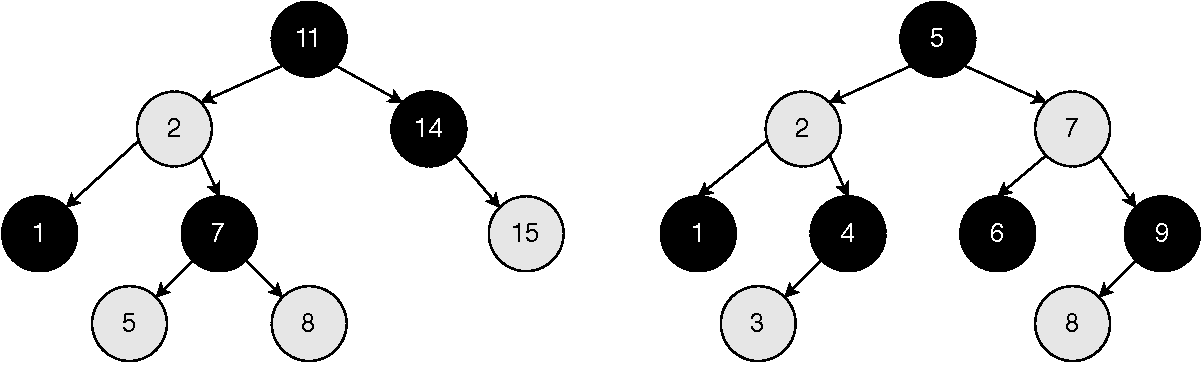
\includegraphics[scale=0.5]{img/imperative-insert}
   \caption{命令式算法构建出的红黑树}
   \label{fig:imperative-insert}
\end{figure}

红黑树的命令式删除算法更为复杂,参见本书附录A。红黑树是一种常见的自平衡二叉树。下一章介绍另外一种自平衡二叉树——AVL树。红黑树可看作其它复杂数据结构的基础:将分枝扩展到$k$个并保持平衡,就演化到B树。将数据存储在边上而非节点中,就演化出基数树。在红黑树的实现中,为了修复平衡性,需要处理多种情况。冈崎给出了一种简化方法,并激发了多种类似的实现\cite{rosetta}。本书中的AVL树、Splay树都是基于模式匹配实现的。

\section{附录:例子程序}

带有父节点引用的红黑树定义,默认节点为红色。

\begin{lstlisting}[language = Bourbaki]
data Node<T> {
    T key
    Color color
    Node<T> left
    Node<T> right
    Node<T> parent

    Node(T x) = Node(null, x, null, Color.RED)

    Node(Node<T> l, T k, Node<T> r, Color c) {
        left = l, key = k, right = r, color = c
        if left != null then left.parent = this
        if right != null then right.parent = this
    }

    Self setLeft(l) {
        left = l
        if l != null then l.parent = this
    }

    Self setRight(r) {
        right = r
        if r != null then r.parent = this
    }

    Node<T> sibling() = if parent.left == this then parent.right
                        else parent.left

    Node<T> uncle() = parent.sibling()

    Node<T> grandparent() = parent.parent
}
\end{lstlisting}

红黑树的插入:

\begin{lstlisting}[language = Bourbaki]
Node<T> insert(Node<T> t, T key) {
    root = t
    x = Node(key)
    parent = null
    while (t != null) {
        parent = t
        t = if (key < t.key) then t.left else t.right
    }
    if (parent == null) {    //tree is empty
        root = x
    } else if (key < parent.key) {
        parent.setLeft(x)
    } else {
        parent.setRight(x)
    }
    return insertFix(root, x)
}
\end{lstlisting}

插入后的平衡修复:

\begin{lstlisting}[language = Bourbaki]
// Fix the red->red violation
Node<T> insertFix(Node<T> t, Node<T> x) {
    while (x.parent != null and x.parent.color == Color.RED) {
        if (x.uncle().color == Color.RED) {
            // case 1: ((a:R x:R b) y:B c:R) ==> ((a:R x:B b) y:R c:B)
            x.parent.color = Color.BLACK
            x.grandparent().color = Color.RED
            x.uncle().color = Color.BLACK
            x = x.grandparent()
        } else {
            if (x.parent == x.grandparent().left) {
                if (x == x.parent.right) {
                    // case 2: ((a x:R b:R) y:B c) ==> case 3
                    x = x.parent
                    t = leftRotate(t, x)
                }
                // case 3: ((a:R x:R b) y:B c) ==> (a:R x:B (b y:R c))
                x.parent.color = Color.BLACK
                x.grandparent().color = Color.RED
                t = rightRotate(t, x.grandparent())
            } else {
                if (x == x.parent.left) {
                    // case 2': (a x:B (b:R y:R c)) ==> case 3'
                    x = x.parent
                    t = rightRotate(t, x)
                }
                // case 3': (a x:B (b y:R c:R)) ==> ((a x:R b) y:B c:R)
                x.parent.color = Color.BLACK
                x.grandparent().color = Color.RED
                t = leftRotate(t, x.grandparent())
            }
        }
    }
    t.color = Color.BLACK
    return t
}
\end{lstlisting}

\ifx\wholebook\relax \else
\section{参考答案}
\shipoutAnswer

\begin{thebibliography}{99}

\bibitem{CLRS}
Thomas H. Cormen, Charles E. Leiserson, Ronald L. Rivest and Clifford Stein.
``Introduction to Algorithms, Second Edition''. ISBN:0262032937. The MIT Press. 2001 (《算法导论》中文版)

\bibitem{okasaki}
Chris Okasaki. ``FUNCTIONAL PEARLS Red-Black Trees in a Functional Setting''. J. Functional Programming. 1998

\bibitem{okasaki-blog}
Chris Okasaki. ``Ten Years of Purely Functional Data Structures''. \url{http://okasaki.blogspot.com/2008/02/ten-years-of-purely-functional-data.html}

\bibitem{wiki-rbt}
Wikipedia. ``Red-black tree''. \url{https://en.wikipedia.org/wiki/Red-black_tree}

\bibitem{lyn}
Lyn Turbak. ``Red-Black Trees''. \url{http://cs.wellesley.edu/~cs231/fall01/red-black.pdf} Nov. 2, 2001.

\bibitem{sgi-stl}
SGI STL. \url{http://www.sgi.com/tech/stl/}

\bibitem{rosetta}
Pattern matching. \url{http://rosettacode.org/wiki/Pattern_matching}

\end{thebibliography}

\expandafter\enddocument

\fi
